\section{V3}
\vspace{-0.5cm} 
\begin{multicols}{2}
    \begin{minipage}{\linewidth}
        \subsection{Halbleiter Speicher} 
        \textbf{Zentraler Speicher}
        \begin{itemize}
            \item direkt am Bussystem angeschlossen
        \end{itemize}
        \textbf{Peripherer Speicher}
        \begin{itemize}
            \item über I/O-Schnittstelle angeschlossen
        \end{itemize}
    \end{minipage}
    
    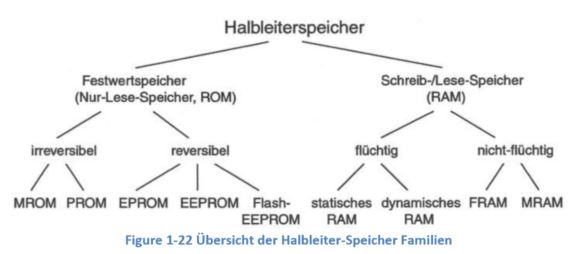
\includegraphics[width=1.1\linewidth]{images/halbleiterfam}
\end{multicols}

\vspace{-1cm} 
\begin{multicols}{2}
    \subsubsection{ROM-Festwertspeicher}
    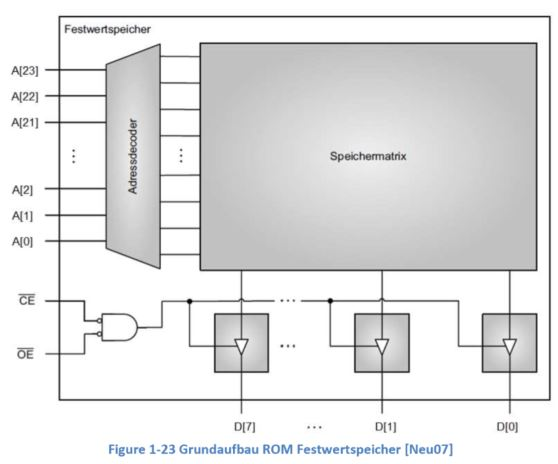
\includegraphics[width=8cm]{images/ROM}
    
    \subsubsection{RAM-Speicher-/Lese-Speicher}
    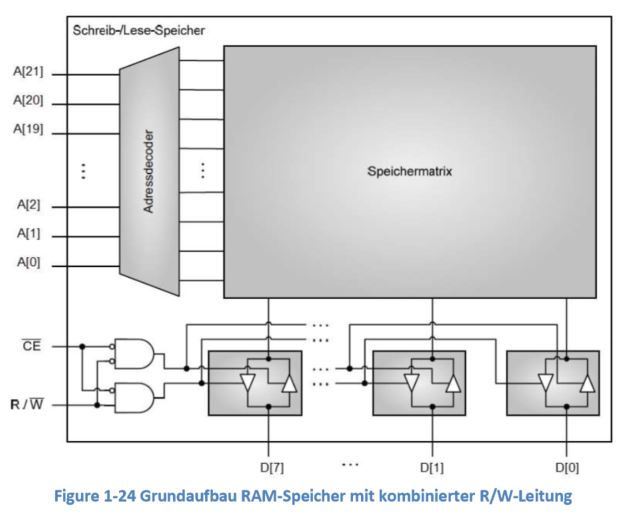
\includegraphics[width=8cm]{images/RAM}
\end{multicols}
    
\vspace{-1cm} 
\subsection{Speicherorganisation}
    
\begin{multicols}{2}
    \subsubsection{Little/Big Endian}
    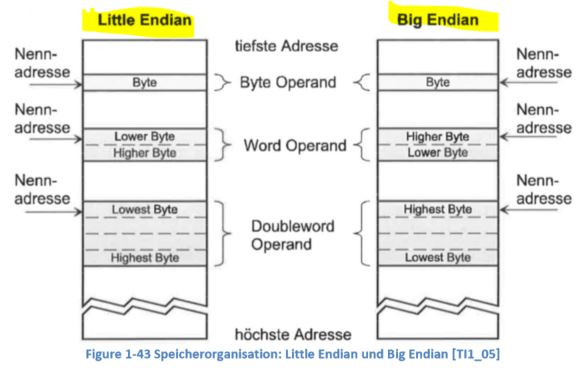
\includegraphics[width=8cm]{images/LittleBigEndian}
    
    \subsubsection{I/O - Schnittstelle}
    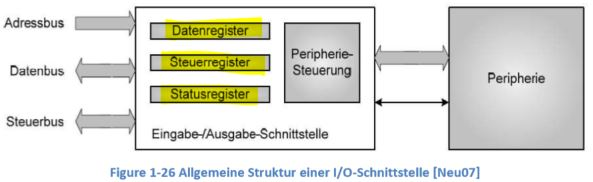
\includegraphics[width=8cm]{images/IOSchnittstelle}
\end{multicols}

\includegraphics[width=12cm]{images/Speicherraumadressierung}
\clearpage
%============================================






















